\section{Conclusions}
Now it's time to draw the line and put everything together. The scope of this section is to highlight important discoveries, results and limitations. \\
The first relevant discovery was understanding the dataset on hand. The dataset contained thick edges that looked like scratches and artifacts from previous layer, so that during the annotation process the current bitmask and previous bitmask had to be used. This lead to the idea of the bitmask integration via the two free color channels and the model became very robust thanks to the additional context information. \\
The first models were very sensitive and the slightest hint of color degradation triggered a false detection. The problem was that the scratches were annotated very inconsistently. Therefore, \textbf{the prominence metric} was developed and it help providing a consistent labeling defined by a clear threshold.\\
Despite this great metric, some images contained nice examples of prominent scratches, but also faded scratches. Now the problem was how to properly filter out those edge cases during development. Here came \textbf{the windowing process} to the rescue, which gave a granular control over the scratch selection of an image by including only the desired windows with prominent scratches. Later on, the lowering of the prominence threshold was possible due to the increased robustness and stability of the model and the model had access to a bit more data. This was only one initial and crucial benefit of windowing. \\
The square shape of the input images avoided unnecessary image padding and toggled the data shuffling on , which removed any concerns regarding the padding methods and made the model overfit less. Also, the smaller windows made the possible to increase the batch size, so that the model can have a more stable batch normalization. \\
The next benefit provided by the windowing technique is the better recall. Because the neighboring windows overlap and also some extra redundant windows gives the model multiple chances to detect the same scratch. \\
The random windowing strategy is relevant for providing variety in the location of the scratches and forces the model to not memorize repetitive and irrelevant structures. On the other hand, the grid strategy might provide repetitive data, but it better suited for the inference task. \\
Another remark is that with windowing before splitting the dataset a better data distribution is obtained. However, it is a better idea to first create the splits and then mix windows between the train and validation split. This way the test dataset can be reconstructed to the original image. This balance of distribution was helpful for a stabilizing the training. \\
With double windowing it has been proved that adding relevant background windows can significantly increase the performance.\\
In order to push down the number of false positives \textbf{the two stage training} approach is used. In the first variant a second class is used to explicitly mark the mistakes from the first training stage. The second variant just introduces the false positive as background windows. This second variant uses also the concept of finding relevant background windows as done with double windowing. The first variant performs better, but tracking the progress during training is difficult, because the extra added class is not an actual class. The second variant deliver also good results, but a bit worse than the first variant, however the upside being that tracking in the second stage is still possible. \\
\textbf{Augmentations} methods help the model to become more robust and overfit less, especially the online augmentations. The first thumb rule is that augmentations that might alter the RGB color channels should be avoided, because they end up modifying the integrated bitmasks. The idea of the bitmasks is that they provide a pixel perfect context information and it makes no sense to alter such information. An exception in this sense might be the contrast augmentation, because the contrast is applied only on the channel that contains the original image. However, the HSV augmentation method can also be applied on the channel with original image, but HSV modifications are not targeted for grayscale images. The second rule of thumb is to avoid occlusions, because it ends up completely or partially covering, which translates to data loss or corruption. If a future dataset contains an amount of images and labels comparable to the open datasets, then occlusions might be a pertinent regularization technique. \\
Some augmentations methods like Mosaic created shorter scratches and previous experiments suggest that training on short scratches makes it more difficult to detect longer scratches. Therefore, a custom online stretching augmentation has been developed to overcome this bias during training. \\
\textbf{Hyperparameters} enhance the results and a small tweak can sometimes have a great impact. The change to an AdamW gradient with a tiny step size of 0.0001 prevented the huge fluctuations of the metrics and losses between epochs. Also, adjusting the weights of the loss functions showed that a trade-off between precision and recall can be obtained. With a strong recall, there was some space to trade-off for a better precision. The box loss was tuned down, so that a good enough localization is provided and the focus is kept on objective and class loss.

\subsection*{Future Work}
All the work generated some nice solutions for the YOLO-based scratch detector. Due to time constraints some limitations still exist and also due to newly released YOLO versions (e.g. YOLOv7) some interesting questions can be posed. \\
A first limitation is posed by the \textbf{constraints of the online augmentations}. In a nutshell, one input images with labels generates exactly one output images with labels of the same size. The only augmentations that can overcome those limitations are some deeply integrated augmentations like Mosaic. Those constraints hold back a stronger random windowing strategy, so that the random windows are generated offline only. An online random windowing process would generate a very strong variance from tiny dataset. \\
A second limitation are the \textbf{fixed 4-windows mosaic augmentation}. More recent papers like \cite{yolo_smoke_paper, improved_mosaic_paper} suggest more complex mosaic variants like a 6-windows or even 9-windows mosaic augmentation. This would surely help with the variance of the data, but this limitation goes hand in hand with the first limitation regarding constraints of online augmentations. Overcoming the first limitation would greatly ease the solving of this second challenge. \\
A third limitation is posed by \textbf{the second stage of the 2 stage training} approach. This is mostly due to the fact that during training metrics are shown as class aggregates and an individual class performance can be seen only at the end. This makes it difficult to get in a comfortable way training metrics. \\
A fourth limitations is posed by \textbf{the small dataset}, but know with the knowledge of labeling the process becomes quicker. An interesting idea would be to run the detection on new images and then to just manually adjust or delete labels, so that the annotation process is sped up. \\
A first possible enhancement would be to experiment with \textbf{alternative loss functions}. In \cite{yolo_smoke_paper} the box tightness and location was improved by replacing the current GIoU functions with Complete Intersection over Union (CIoU) or Distance Intersection Over Union (DIoU). The DIoU is an enhancement of GIoU and CIoU is in turn an enhancement of DIoU, so some improvement would be expected. In the context of multi-class detections, the BCE loss could be replaced with a Categorical Class Entropy (CCE). The BCE is advantageous for multi-labeling of the same object e.g. the labels \textit{dog} and \textit{animal} can be used to label a dog. In the current situation the labels are multi-exclusive by being a scratch or a false positive from the first training stage, so the CCE might help the model better distinguish classes. \\
A second possible enhancement would be to change the hardcoded values for the \textbf{metrics during training}. More specifically, it would be nice to get also the mAP at lower threshold like 0.4 during training. This is helpful in the beginning when the model is able to correctly identify the scratches, but due to a bad localization the IoU often slightly under 0.5. Therefore, it was difficult to tell without manual intervention, if the model failed to completely detect scratches or if the localization was bad during training. \\
A third possible more complex enhancement would be to upgrade to the new \textbf{YOLOv7}. This change opens the doors to many new possibilities and improvements. YOLOv7 is currently in it's early stages, but the team behind this project is a reputable team that developed the YOLOv1-4 versions.\\
 YOLOv7 also allows a new type of labels called \textbf{keypoints}. An example of keypoints can be seen in figure \ref{conc:yolov7_kp_annot}.

 \begin{figure}[!h]
   \centering
   \captionsetup{justification=centering,margin=2cm}
   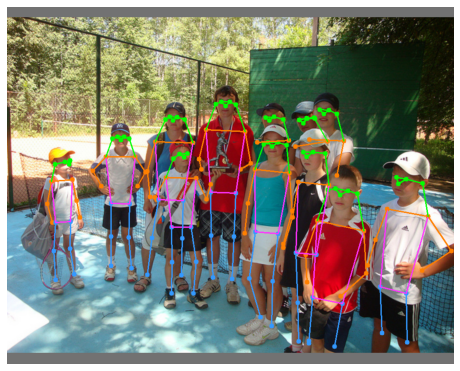
\includegraphics[width=0.75\columnwidth]{images/conclusions/yolov7_keypoints}
   \caption{YOLOv7 keypoint annotations}
   \label{conc:yolov7_kp_annot}
 \end{figure}

An interesting idea would be to replace the bounding boxes of the scratches with 2 keypoints. The idea of using bounding boxes was that it simplifies the labeling process and it also removes the need of pixel perfect labeling. In the same direction would be the usage of keypoints, because there will no more worries regarding the width of the bounding box. This dimensionality reduction might remove important data captured by the bounding boxes. \\


 \begin{figure}[!h]
   \centering
   \captionsetup{justification=centering,margin=2cm}
   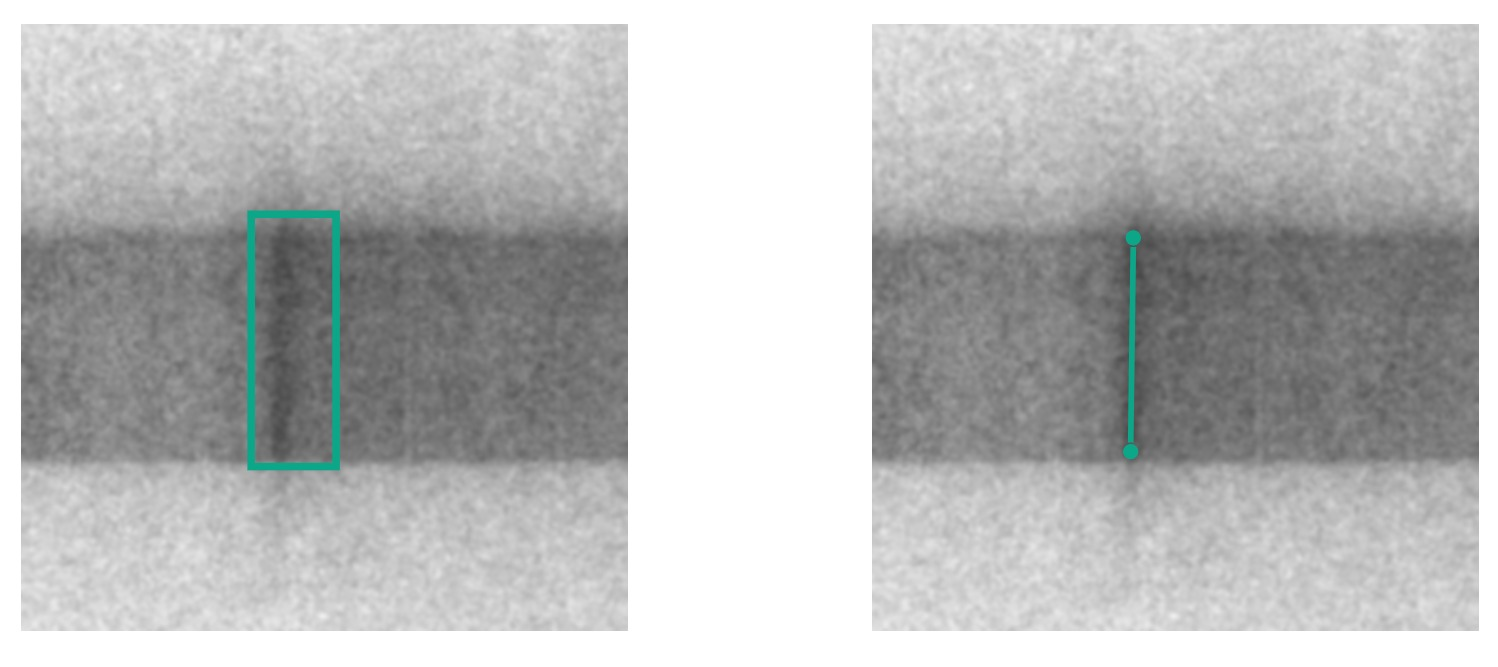
\includegraphics[width=0.75\columnwidth]{images/conclusions/bb_vs_kp_annot}
   \caption{Alternative annotations}
   \label{conc:bb_vs_kp}
 \end{figure}
